%% ============================================================
%% SAMBPS — Self-Adaptive Model-Based Protection Systems
%% Correlation with IEEE Std C37.300-2024 (CPC Systems)
%%
%% Audience  : Protection Engineers, Researchers
%% Author    : Anoop V. Eluvathingal, IIT Madras
%% Supervisor: Prof. K. Shanti Swarup
%% Date      : April 2026
%%
%% Compile   : pdflatex sambps_cpc.tex (twice)
%%
%% SPEAKER NOTES
%%   Notes are embedded using \note{...}.
%%   To produce a notes-only PDF for printing, uncomment:
%%     \setbeameroption{show only notes}
%%   To show notes alongside slides (dual monitor):
%%     \setbeameroption{show notes on second screen=right}
%%   Default (commented): slides only.
%% ============================================================
\documentclass[aspectratio=169, 10pt]{beamer}

%% ── Speaker notes ───────────────────────────────────────────
\usepackage{pgfpages}
%\setbeameroption{show only notes}
%\setbeameroption{show notes on second screen=right}

%% ── Packages ────────────────────────────────────────────────
\usepackage{tikz}
\usepackage{pgfplots}
\pgfplotsset{compat=1.18}
\usetikzlibrary{%
  shapes, shapes.geometric, arrows, arrows.meta,
  calc, positioning, fit, matrix,
  decorations.pathreplacing, decorations.markings, patterns,
}
\usepackage{amsmath, amssymb, bm}
\usepackage{booktabs}
\usepackage{array, multirow, tabularx}
\usepackage[table]{xcolor}
\usepackage{colortbl}
\usepackage{graphicx}
\usepackage{tcolorbox}
\tcbuselibrary{skins, breakable}
\usepackage{pifont}
\usepackage{siunitx}

%% ── Colour palette ──────────────────────────────────────────
\definecolor{iitmMaroon}  {RGB}{128,  0,  0}
\definecolor{iitmGold}    {RGB}{179,145, 25}
\definecolor{iitmDarkBlue}{RGB}{ 15, 45, 90}
\definecolor{iitmLightBg} {RGB}{248,244,240}
\definecolor{thesisblue}  {RGB}{  0, 70,140}
\definecolor{thesisred}   {RGB}{180, 30, 30}
\definecolor{thesisgreen} {RGB}{ 20,120, 60}
\definecolor{thesisorange}{RGB}{200, 90,  0}
\definecolor{thesisgray}  {RGB}{100,100,110}
\definecolor{thesisteal}  {RGB}{  0,130,130}
\definecolor{thesispurple}{RGB}{100,  0,150}
\definecolor{lightblue}   {RGB}{220,235,255}
\definecolor{lightgreen}  {RGB}{220,245,225}
\definecolor{lightorange} {RGB}{255,240,220}
\definecolor{lightyellow} {RGB}{255,252,220}
\definecolor{lightgray}   {RGB}{240,240,242}
\definecolor{passpink}    {RGB}{255,245,245}
\definecolor{passgreen}   {RGB}{235,252,235}
\definecolor{cpcblue}     {RGB}{  0, 90,160}
\definecolor{cpcgreen}    {RGB}{ 10,110, 50}

%% ── Beamer theme ────────────────────────────────────────────
\usetheme{default}
\usecolortheme[named=iitmMaroon]{structure}

\setbeamercolor{palette primary}   {bg=iitmMaroon,   fg=white}
\setbeamercolor{palette secondary} {bg=iitmMaroon,   fg=white}
\setbeamercolor{frametitle}        {bg=iitmMaroon,   fg=white}
\setbeamercolor{title}             {fg=white,        bg=iitmMaroon}
\setbeamercolor{block title}       {fg=white,        bg=iitmDarkBlue}
\setbeamercolor{block body}        {bg=iitmLightBg}
\setbeamercolor{alerted text}      {fg=iitmMaroon}
\setbeamercolor{background canvas} {bg=white}
\setbeamerfont{frametitle}{size=\large, series=\bfseries}
\setbeamerfont{title}     {size=\Large, series=\bfseries}
\setbeamertemplate{navigation symbols}{}

%% Frametitle: full-width maroon bar
\setbeamertemplate{frametitle}{%
  \nointerlineskip%
  \begin{beamercolorbox}[wd=\paperwidth,ht=0.92cm,dp=0.13cm,
                          leftskip=0.55cm,rightskip=0.4cm]{frametitle}%
    \vbox to 0.92cm{\vfil%
      \usebeamerfont{frametitle}\usebeamercolor[fg]{frametitle}%
      \insertframetitle%
    \vfil}%
  \end{beamercolorbox}%
}

%% Footline: maroon bar
\setbeamertemplate{footline}{%
  \leavevmode%
  \begin{beamercolorbox}[wd=\paperwidth,ht=0.48cm,dp=0.12cm]{palette primary}%
    \hspace{0.45cm}%
    {\scriptsize\color{white}%
      A.\,V.\,Eluvathingal \enspace|\enspace
      SAMBPS \& IEEE C37.300-2024 CPC Correlation \enspace|\enspace
      IIT Madras}%
    \hfill%
    {\scriptsize\color{white}%
      \insertframenumber/\inserttotalframenumber%
      \hspace{0.45cm}}%
  \end{beamercolorbox}%
}

%% ── Macros ──────────────────────────────────────────────────
\newcommand{\SAMBPS}{\textsc{sambps}}
\newcommand{\pu}{\,\text{p.u.}}
\newcommand{\ms}{\,\text{ms}}
\newcommand{\Hz}{\,\text{Hz}}
\newcommand{\kIBR}{k_{\rm ibr}}
\newcommand{\kn}{\kappa_n}
\newcommand{\cmark}{\textcolor{thesisgreen}{\ding{51}}}
\newcommand{\xmark}{\textcolor{thesisred}{\ding{55}}}
\newcommand{\PD}{P_D}
\newcommand{\PFA}{P_{FA}}
\newcommand{\CPC}{\textsc{cpc}}

%% Result highlight box
\tcbset{
  resultbox/.style={
    enhanced, boxrule=0.8pt, arc=3pt,
    colback=passgreen, colframe=thesisgreen,
    fonttitle=\bfseries\footnotesize, coltitle=white,
    attach boxed title to top left={yshift=-2mm, xshift=3mm},
    boxed title style={colback=thesisgreen, arc=2pt},
    left=2mm, right=2mm, top=2mm, bottom=2mm,
  },
  warnbox/.style={
    enhanced, boxrule=0.8pt, arc=3pt,
    colback=lightorange, colframe=thesisorange,
    fonttitle=\bfseries\footnotesize, coltitle=white,
    attach boxed title to top left={yshift=-2mm, xshift=3mm},
    boxed title style={colback=thesisorange, arc=2pt},
    left=2mm, right=2mm, top=2mm, bottom=2mm,
  },
  keybox/.style={
    enhanced, boxrule=0.8pt, arc=3pt,
    colback=lightblue, colframe=thesisblue,
    left=2mm, right=2mm, top=1.5mm, bottom=1.5mm,
  },
  cpcbox/.style={
    enhanced, boxrule=0.9pt, arc=3pt,
    colback=lightblue!60, colframe=cpcblue,
    fonttitle=\bfseries\scriptsize, coltitle=white,
    attach boxed title to top left={yshift=-2mm, xshift=3mm},
    boxed title style={colback=cpcblue, arc=2pt},
    left=2mm, right=2mm, top=2mm, bottom=2mm,
  },
}

%% ── Title metadata ──────────────────────────────────────────
\title[\SAMBPS{} \textbar\ CPC Correlation]{%
  \textbf{Self-Adaptive Model-Based Protection Systems}\\[4pt]
  {\large Highlights, Results, and Correlation with\\
  IEEE Std C37.300-2024 Centralised Protection \& Control}}

\author[A.\,V.\,Eluvathingal \& K.\,S.\,Swarup]{%
  \textbf{Anoop V.\ Eluvathingal}\quad|\quad
  Supervisor: Prof.\ K.\ Shanti Swarup\\[2pt]
  {\small Department of Electrical Engineering,
    Indian Institute of Technology Madras, Chennai~600\,036, India}}

\date{April 2026}

%% ============================================================
\begin{document}
%% ============================================================

%% ── Title slide ─────────────────────────────────────────────
{%
\setbeamertemplate{footline}{}
\begin{frame}[plain]
  \begin{tikzpicture}[remember picture, overlay]
    %% Background panel
    \fill[iitmMaroon] (current page.north west) rectangle
                      ([yshift=-3.0cm]current page.north east);
    %% IIT Madras label top-right
    \node[anchor=north east, font=\scriptsize\bfseries, text=iitmGold]
      at ([xshift=-0.5cm, yshift=-0.18cm]current page.north east)
      {Indian Institute of Technology Madras};
    %% Title block
    \node[anchor=center, align=center, text=white,
          font=\bfseries\large, text width=14cm]
      at ([yshift=-1.48cm]current page.north)
      {\textbf{Self-Adaptive Model-Based Protection Systems}\\[6pt]
       {\normalsize Highlights, Results, and Correlation with\\
        IEEE Std C37.300-2024 Centralised Protection \& Control}};
    %% Author block
    \node[anchor=center, align=center, text=iitmDarkBlue,
          font=\small, text width=14cm]
      at (current page.center)
      {\textbf{Anoop V.\ Eluvathingal} \quad|\quad
       Supervisor: Prof.\ K.\ Shanti Swarup\\[3pt]
       Department of Electrical Engineering\\
       Indian Institute of Technology Madras, Chennai~600\,036, India};
    %% Date and venue
    \node[anchor=south, align=center, text=thesisgray, font=\footnotesize]
      at ([yshift=1.0cm]current page.south)
      {April 2026};
    %% Bottom accent line
    \draw[iitmGold, line width=2pt]
      ([yshift=0.7cm]current page.south west) --
      ([yshift=0.7cm]current page.south east);
    %% C37.300 badge
    \node[anchor=south east, align=center, font=\tiny\bfseries,
          text=cpcblue, text width=3.2cm]
      at ([xshift=-0.5cm, yshift=0.75cm]current page.south east)
      {Correlated with\\IEEE Std C37.300-2024};
  \end{tikzpicture}
\end{frame}
}

%% ── Slide 2: Outline ─────────────────────────────────────────
\begin{frame}{Presentation Outline}
\vspace{-4pt}
\begin{columns}[T]
\column{0.48\textwidth}
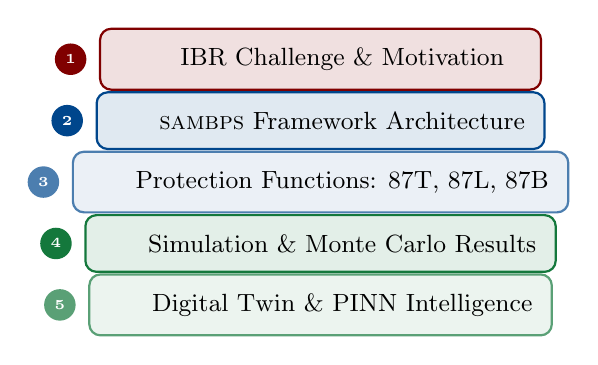
\begin{tikzpicture}[
  sec/.style={rectangle, rounded corners=4pt, minimum width=5.6cm,
    minimum height=0.72cm, align=left, font=\small, line width=0.8pt,
    inner sep=7pt},
  num/.style={circle, minimum size=0.40cm, font=\bfseries\tiny,
    text=white, inner sep=0pt},
]
\node[sec, fill=iitmMaroon!12, draw=iitmMaroon](S1) at (0, 3.4)
  {\hspace{0.55cm}IBR Challenge \& Motivation};
\node[sec, fill=thesisblue!12, draw=thesisblue](S2) at (0, 2.62)
  {\hspace{0.55cm}\SAMBPS{} Framework Architecture};
\node[sec, fill=thesisblue!8, draw=thesisblue!70](S3) at (0, 1.84)
  {\hspace{0.55cm}Protection Functions: 87T, 87L, 87B};
\node[sec, fill=thesisgreen!12, draw=thesisgreen](S4) at (0, 1.06)
  {\hspace{0.55cm}Simulation \& Monte Carlo Results};
\node[sec, fill=thesisgreen!8, draw=thesisgreen!70](S5) at (0, 0.28)
  {\hspace{0.55cm}Digital Twin \& PINN Intelligence};

\node[num, fill=iitmMaroon]   at ($(S1.west)+(-0.36,0)$) {1};
\node[num, fill=thesisblue]   at ($(S2.west)+(-0.36,0)$) {2};
\node[num, fill=thesisblue!70]at ($(S3.west)+(-0.36,0)$) {3};
\node[num, fill=thesisgreen]  at ($(S4.west)+(-0.36,0)$) {4};
\node[num, fill=thesisgreen!70]at($(S5.west)+(-0.36,0)$) {5};
\end{tikzpicture}

\column{0.48\textwidth}
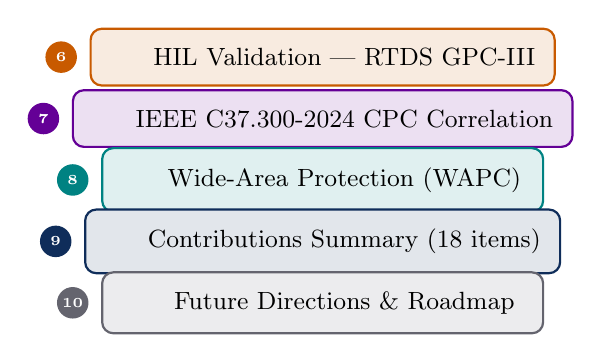
\begin{tikzpicture}[
  sec/.style={rectangle, rounded corners=4pt, minimum width=5.6cm,
    minimum height=0.72cm, align=left, font=\small, line width=0.8pt,
    inner sep=7pt},
  num/.style={circle, minimum size=0.40cm, font=\bfseries\tiny,
    text=white, inner sep=0pt},
]
\node[sec, fill=thesisorange!12, draw=thesisorange](S6) at (0, 3.4)
  {\hspace{0.55cm}HIL Validation --- RTDS GPC-III};
\node[sec, fill=thesispurple!12, draw=thesispurple](S7) at (0, 2.62)
  {\hspace{0.55cm}IEEE C37.300-2024 CPC Correlation};
\node[sec, fill=thesisteal!12, draw=thesisteal](S8) at (0, 1.84)
  {\hspace{0.55cm}Wide-Area Protection (WAPC)};
\node[sec, fill=iitmDarkBlue!12, draw=iitmDarkBlue](S9) at (0, 1.06)
  {\hspace{0.55cm}Contributions Summary (18 items)};
\node[sec, fill=thesisgray!12, draw=thesisgray](S10) at (0, 0.28)
  {\hspace{0.55cm}Future Directions \& Roadmap};

\node[num, fill=thesisorange]  at ($(S6.west)+(-0.36,0)$) {6};
\node[num, fill=thesispurple]  at ($(S7.west)+(-0.36,0)$) {7};
\node[num, fill=thesisteal]    at ($(S8.west)+(-0.36,0)$) {8};
\node[num, fill=iitmDarkBlue]  at ($(S9.west)+(-0.36,0)$) {9};
\node[num, fill=thesisgray]    at ($(S10.west)+(-0.36,0)$){10};
\end{tikzpicture}
\end{columns}
\note{10-section presentation covering all aspects of SAMBPS, from the fundamental IBR challenge through to the IEEE C37.300 CPC correlation. Approximately 40 minutes including discussion.}
\end{frame}

%% ── Slide 3: IBR Challenge ───────────────────────────────────
\begin{frame}{Context: Why IBR-Dominated Networks Break Classical Protection}
\vspace{-4pt}
\begin{columns}[T]
\column{0.50\textwidth}
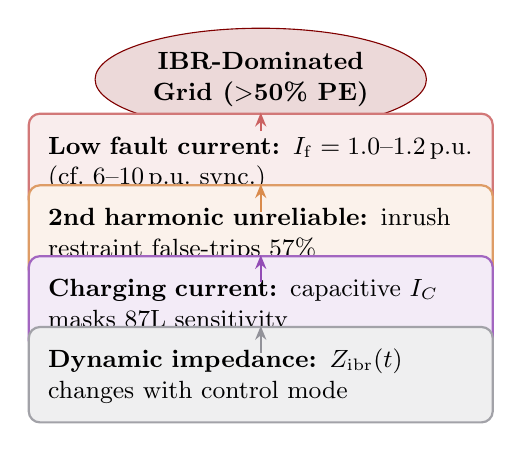
\begin{tikzpicture}[
  prob/.style={rectangle, rounded corners=4pt, minimum width=5.8cm,
    minimum height=0.82cm, align=left, font=\small\strut, line width=0.8pt,
    inner sep=7pt},
  arr/.style={-{Stealth[length=5pt,width=4pt]}, line width=0.9pt},
]
%% Central IBR node
\node[ellipse, fill=iitmMaroon!15, draw=iitmMaroon, minimum width=3.2cm,
      minimum height=0.9cm, font=\small\bfseries, align=center]
  (IBR) at (0, 3.0) {IBR-Dominated\\Grid ($>$50\% PE)};

%% Four failure modes
\node[prob, fill=thesisred!8, draw=thesisred!60, text width=5.4cm]
  (F1) at (0, 1.95) {\textbf{Low fault current:}
    $I_{\rm f} = 1.0$--$1.2\pu$ (cf.\ 6--10$\pu$ sync.)};
\node[prob, fill=thesisorange!8, draw=thesisorange!60, text width=5.4cm]
  (F2) at (0, 1.05) {\textbf{2nd harmonic unreliable:}
    inrush restraint false-trips 57\%};
\node[prob, fill=thesispurple!8, draw=thesispurple!60, text width=5.4cm]
  (F3) at (0, 0.15) {\textbf{Charging current:}
    capacitive $I_C$ masks 87L sensitivity};
\node[prob, fill=thesisgray!10, draw=thesisgray!60, text width=5.4cm]
  (F4) at (0,-0.75) {\textbf{Dynamic impedance:}
    $Z_{\rm ibr}(t)$ changes with control mode};

\draw[arr, thesisred!70]    (IBR.south) -- (F1.north);
\draw[arr, thesisorange!70] (F1.south) -- (F2.north);
\draw[arr, thesispurple!70] (F2.south) -- (F3.north);
\draw[arr, thesisgray!70]   (F3.south) -- (F4.north);
\end{tikzpicture}

\column{0.46\textwidth}
\vspace{6pt}
\begin{tcolorbox}[warnbox, title={The Core Problem}]
{\small Classical threshold-based relays were designed for synchronous generators.
In IBR-dominated grids, fault signatures \emph{lie within normal operating bands}
--- rendering fixed-threshold detection unreliable.}
\end{tcolorbox}
\vspace{6pt}
\begin{tcolorbox}[keybox]
{\small\textbf{SAMBPS answer:} Replace fixed thresholds with a
\emph{self-adaptive} 5-layer model-based architecture that
tracks IBR operating state in real time.}
\end{tcolorbox}
\vspace{8pt}
{\footnotesize
\begin{tabular}{lcc}
\toprule
\textbf{Metric} & \textbf{Conventional} & \textbf{SAMBPS}\\
\midrule
87T false-trip (inrush) & 57\% & $<$0.1\%\\
87L detect ($I_f$=0.1\pu) & Fail & \cmark\\
87B coordination CTI    & 0    & 100\%\\
Fault location error     & ---  & $\le$2.4\%\\
\bottomrule
\end{tabular}}
\end{columns}
\note{Set the scene: inverter-based resources (solar PV, wind DFIG, BESS) now dominate many grids and their fault behaviour is fundamentally different from synchronous generators. The four failure modes shown are all demonstrated quantitatively in the SAMBPS thesis work. The table numbers come directly from Monte Carlo studies with 30,000 scenarios.}
\end{frame}

%% ── Slide 4: SAMBPS Architecture ────────────────────────────
\begin{frame}{\SAMBPS{} --- Five-Layer Self-Adaptive Architecture}
\vspace{-6pt}
\begin{center}
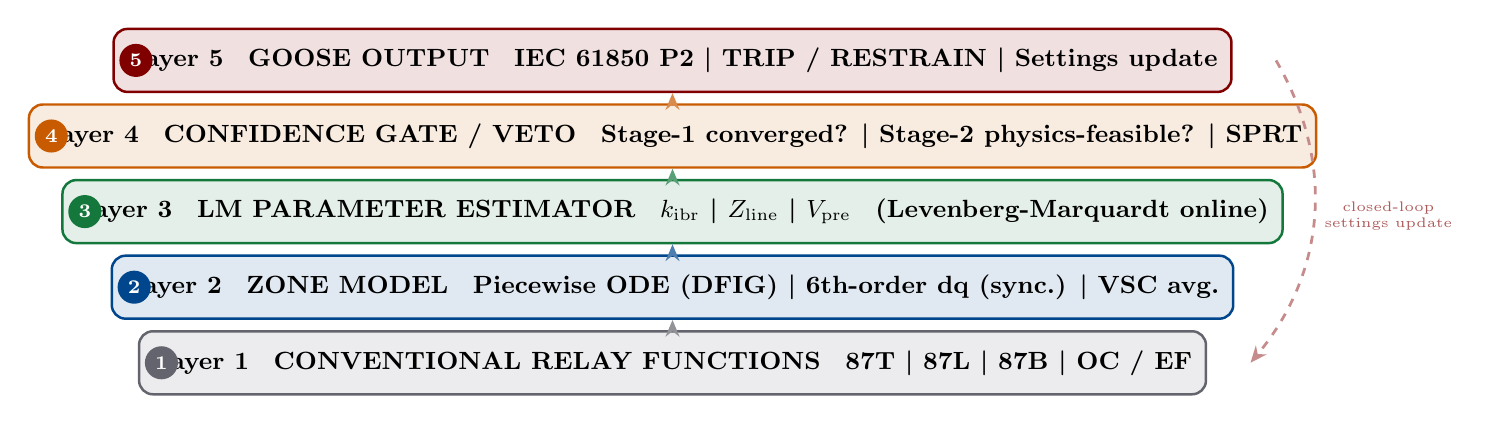
\begin{tikzpicture}[
  layer/.style={rectangle, rounded corners=5pt, minimum width=11.0cm,
    minimum height=0.80cm, align=center, font=\small\bfseries,
    line width=0.9pt, inner sep=5pt},
  lnum/.style={circle, minimum size=0.42cm, font=\bfseries\scriptsize,
    text=white, inner sep=0pt},
  arr/.style={-{Stealth[length=6pt,width=5pt]}, line width=1.0pt},
]
%% Five layers (bottom-up)
\node[layer, fill=thesisgray!12, draw=thesisgray]
  (L1) at (0, 0.0) {Layer~1 \enspace CONVENTIONAL RELAY FUNCTIONS \enspace
    87T \textbar\ 87L \textbar\ 87B \textbar\ OC / EF};
\node[layer, fill=thesisblue!12, draw=thesisblue]
  (L2) at (0, 0.96) {Layer~2 \enspace ZONE MODEL
    \enspace Piecewise ODE (DFIG) \textbar\ 6th-order dq (sync.) \textbar\ VSC avg.};
\node[layer, fill=thesisgreen!12, draw=thesisgreen]
  (L3) at (0, 1.92) {Layer~3 \enspace LM PARAMETER ESTIMATOR
    \enspace $\kIBR$ \textbar\ $Z_{\rm line}$ \textbar\ $V_{\rm pre}$
    \enspace (Levenberg-Marquardt online)};
\node[layer, fill=thesisorange!12, draw=thesisorange]
  (L4) at (0, 2.88) {Layer~4 \enspace CONFIDENCE GATE / VETO
    \enspace Stage-1 converged? \textbar\ Stage-2 physics-feasible? \textbar\ SPRT};
\node[layer, fill=iitmMaroon!12, draw=iitmMaroon]
  (L5) at (0, 3.84) {Layer~5 \enspace GOOSE OUTPUT
    \enspace IEC~61850 P2 \textbar\ TRIP / RESTRAIN \textbar\ Settings update};

%% Layer numbers (inset on left edge of each layer)
\node[lnum, fill=thesisgray]   at ($(L1.west)+(0.30,0)$) {1};
\node[lnum, fill=thesisblue]   at ($(L2.west)+(0.30,0)$) {2};
\node[lnum, fill=thesisgreen]  at ($(L3.west)+(0.30,0)$) {3};
\node[lnum, fill=thesisorange] at ($(L4.west)+(0.30,0)$) {4};
\node[lnum, fill=iitmMaroon]   at ($(L5.west)+(0.30,0)$) {5};

%% Upward flow arrows (between layers, centred)
\draw[arr, thesisgray!70]   (L1.north) -- (L2.south);
\draw[arr, thesisblue!70]   (L2.north) -- (L3.south);
\draw[arr, thesisgreen!70]  (L3.north) -- (L4.south);
\draw[arr, thesisorange!70] (L4.north) -- (L5.south);

%% Feedback arrow: right side, using calc so no overlay trigger
\draw[arr, iitmMaroon!45, dashed, bend left=35]
  ($(L5.east)+(0.55,0)$) to node[anchor=west, font=\tiny, text=iitmMaroon!65,
    align=center] {closed-loop\\settings update}
  ($(L1.east)+(0.55,0)$);
\end{tikzpicture}
\end{center}
\note{The 5-layer architecture is the central design principle. Layers 1-2 are classical; Layers 3-5 are what make SAMBPS adaptive. The feedback arrow from L5 back to L1 represents the closed-loop adaptive settings update --- this is what enables the system to self-tune as IBR operating conditions change. All five layers run as a Python IED communicating via IEC 61850 GOOSE.}
\end{frame}

%% ── Slide 5: Protection Functions 87T ───────────────────────
\begin{frame}{Protection Function: 87T --- Bayesian SPRT Inrush Discrimination}
\vspace{-4pt}
\begin{columns}[T]
\column{0.52\textwidth}
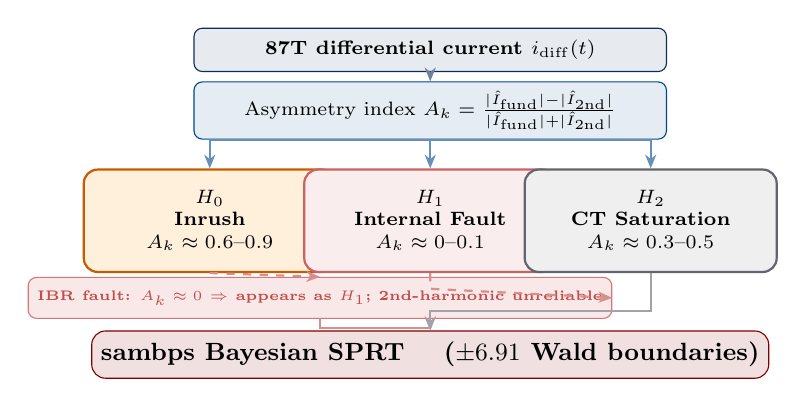
\begin{tikzpicture}[
  hyp/.style={rectangle, rounded corners=5pt, minimum width=3.2cm,
    minimum height=1.30cm, align=center, font=\scriptsize,
    line width=0.8pt, inner sep=5pt},
  dec/.style={rectangle, rounded corners=3pt, minimum width=1.8cm,
    minimum height=0.55cm, align=center, font=\scriptsize\bfseries,
    line width=0.8pt},
  arr/.style={-{Stealth[length=5pt,width=4pt]}, line width=0.8pt},
]
%% Signal input
\node[rectangle, rounded corners=3pt, fill=iitmDarkBlue!10,
      draw=iitmDarkBlue, minimum width=6.0cm, minimum height=0.55cm,
      font=\scriptsize\bfseries, align=center]
  (SIG) at (0, 3.35) {87T differential current $i_{\rm diff}(t)$};
%% Asymmetry index
\node[rectangle, rounded corners=3pt, fill=thesisblue!10,
      draw=thesisblue, minimum width=6.0cm, minimum height=0.62cm,
      font=\scriptsize, align=center]
  (AK) at (0, 2.58)
  {Asymmetry index $A_k = \frac{|\hat{I}_{\rm fund}| - |\hat{I}_{\rm 2nd}|}%
   {|\hat{I}_{\rm fund}| + |\hat{I}_{\rm 2nd}|}$};
\draw[arr, iitmDarkBlue!60] (SIG.south) -- (AK.north);

%% Three hypotheses
\node[hyp, fill=lightorange, draw=thesisorange]
  (H0) at (-2.8, 1.18)
  {$H_0$\\\textbf{Inrush}\\$A_k \approx 0.6$--$0.9$};
\node[hyp, fill=thesisred!8, draw=thesisred!70]
  (H1) at (0, 1.18)
  {$H_1$\\\textbf{Internal Fault}\\$A_k \approx 0$--$0.1$};
\node[hyp, fill=thesisgray!10, draw=thesisgray]
  (H2) at (2.8, 1.18)
  {$H_2$\\\textbf{CT Saturation}\\$A_k \approx 0.3$--$0.5$};

\draw[arr, thesisblue!60] (AK.south) -| (H0.north);
\draw[arr, thesisblue!60] (AK.south) -- (H1.north);
\draw[arr, thesisblue!60] (AK.south) -| (H2.north);

%% IBR confusion box
\node[rectangle, rounded corners=3pt, fill=thesisred!10,
      draw=thesisred!60, minimum width=5.8cm, minimum height=0.52cm,
      font=\tiny\bfseries, align=center, text=thesisred!80]
  (IBR) at (-1.4, 0.20)
  {IBR fault: $A_k \approx 0$ $\Rightarrow$ appears as $H_1$; 2nd-harmonic unreliable};
\draw[arr, thesisred!50, dashed] (H0.south) -- (IBR.north);
\draw[arr, thesisred!50, dashed] (H1.south) -- ++(0,-0.2) -- (IBR.east);

%% SPRT decision
\node[rectangle, rounded corners=5pt, fill=iitmMaroon!12,
      draw=iitmMaroon, minimum width=6.0cm, minimum height=0.60cm,
      font=\small\bfseries, align=center]
  (SPRT) at (0, -0.52)
  {\SAMBPS{} Bayesian SPRT \quad ($\pm 6.91$ Wald boundaries)};
\draw[arr, thesisred!50] (IBR.south) -- ++(0,-0.12) -| (SPRT.north);
\draw[arr, thesisgray!60] (H2.south) -- ++(0,-0.48) -| (SPRT.north);
\end{tikzpicture}

\column{0.44\textwidth}
\vspace{4pt}
\begin{tcolorbox}[resultbox, title={Monte Carlo Results (30k scenarios)}]
{\footnotesize
\begin{tabular}{lc}
\toprule
\textbf{Metric} & \textbf{SAMBPS}\\
\midrule
$\PD$ (internal fault)     & \textbf{1.000}\\
$\PFA$ (false trip)        & $<$0.001\\
Inrush block accuracy      & 99.9\%\\
IBR scenarios covered      & DFIG, PV, VSC\\
Avg.\ decision time        & $\le$22\ms\\
\bottomrule
\end{tabular}}
\end{tcolorbox}
\vspace{6pt}
\begin{tcolorbox}[keybox]
{\scriptsize\textbf{Key innovation:} Three-hypothesis SPRT replaces
single-threshold 2nd-harmonic restraint. Works even when IBR
drives $A_k$ into the inrush band.}
\end{tcolorbox}
\vspace{4pt}
{\scriptsize\textbf{Stage-2 veto gate:} Physics-feasibility check
prevents mal-operation when LM estimator has not converged ($\kIBR$
uncertainty $>$5\%).}
\end{columns}
\note{The SPRT approach uses sequential probability ratio testing with Wald boundaries at +6.91 (trip) and -6.91 (block). The three-hypothesis formulation is the key novelty over classical two-class SPRT. The 30,000 Monte Carlo scenarios span all IBR types (DFIG, PV, VSC) across a range of fault impedances, fault angles, and pre-fault loading conditions.}
\end{frame}

%% ── Slide 6: 87L Five-Element Chain ─────────────────────────
\begin{frame}[t]{Protection Function: 87L --- Five-Element IBR-Adaptive Line Chain}
\vspace{-4pt}
\begin{columns}[T]
\column{0.54\textwidth}
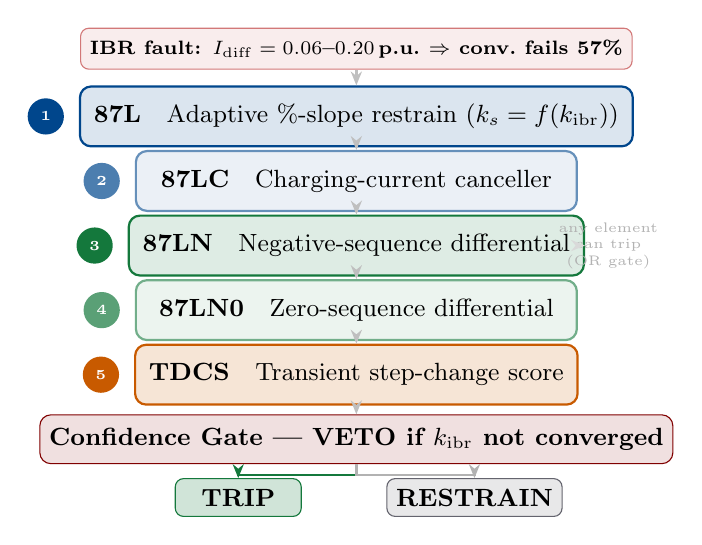
\begin{tikzpicture}[
  el/.style={rectangle, rounded corners=4pt, minimum width=5.6cm,
    minimum height=0.76cm, align=center, font=\small,
    line width=0.8pt, inner sep=5pt},
  badge/.style={circle, minimum size=0.46cm,
    font=\bfseries\tiny, text=white, inner sep=0pt},
  farr/.style={-{Stealth[length=5pt,width=4pt]}, line width=0.9pt},
]
%% Problem banner
\node[rectangle, rounded corners=3pt, fill=thesisred!8,
      draw=thesisred!60, minimum width=5.6cm, minimum height=0.52cm,
      font=\scriptsize\bfseries, align=center]
  (prob) at (0, 3.60)
  {IBR fault: $I_{\mathrm{diff}}=0.06$--$0.20\pu$ $\Rightarrow$ conv.\ fails 57\%};

\node[el, fill=thesisblue!14, draw=thesisblue]
  (E1) at (0, 2.74) {\textbf{87L}\quad Adaptive \%-slope restrain ($k_s = f(\kIBR)$)};
\node[el, fill=thesisblue!8, draw=thesisblue!60]
  (E2) at (0, 1.92) {\textbf{87LC}\quad Charging-current canceller};
\node[el, fill=thesisgreen!14, draw=thesisgreen]
  (E3) at (0, 1.10) {\textbf{87LN}\quad Negative-sequence differential};
\node[el, fill=thesisgreen!8, draw=thesisgreen!60]
  (E4) at (0, 0.28) {\textbf{87LN0}\quad Zero-sequence differential};
\node[el, fill=thesisorange!16, draw=thesisorange]
  (E5) at (0,-0.54) {\textbf{TDCS}\quad Transient step-change score};

\node[badge, fill=thesisblue]     at ($(E1.west)+(-0.42,0)$) {1};
\node[badge, fill=thesisblue!70]  at ($(E2.west)+(-0.42,0)$) {2};
\node[badge, fill=thesisgreen]    at ($(E3.west)+(-0.42,0)$) {3};
\node[badge, fill=thesisgreen!70] at ($(E4.west)+(-0.42,0)$) {4};
\node[badge, fill=thesisorange]   at ($(E5.west)+(-0.42,0)$) {5};

%% Confidence gate
\node[rectangle, rounded corners=4pt, fill=iitmMaroon!12,
      draw=iitmMaroon, minimum width=5.6cm, minimum height=0.62cm,
      font=\small\bfseries, align=center]
  (CG) at (0,-1.36) {Confidence Gate --- VETO if $\kIBR$ not converged};
\node[rectangle, rounded corners=3pt, fill=thesisgreen!20,
      draw=thesisgreen, minimum width=1.6cm, minimum height=0.48cm,
      font=\small\bfseries, align=center]
  (TRIP) at (-1.5,-2.10) {TRIP};
\node[rectangle, rounded corners=3pt, fill=thesisgray!15,
      draw=thesisgray, minimum width=1.6cm, minimum height=0.48cm,
      font=\small\bfseries, align=center]
  (REST) at (1.5,-2.10) {RESTRAIN};

\draw[farr, gray!50] (prob.south) -- (E1.north);
\draw[farr, gray!50] (E1.south) -- (E2.north);
\draw[farr, gray!50] (E2.south) -- (E3.north);
\draw[farr, gray!50] (E3.south) -- (E4.north);
\draw[farr, gray!50] (E4.south) -- (E5.north);
\draw[farr, gray!50] (E5.south) -- (CG.north);
\draw[farr, thesisgreen] (CG.south) -- ++(0,-0.14) -| (TRIP.north);
\draw[farr, gray!60]     (CG.south) -- ++(0,-0.14) -| (REST.north);

%% OR annotation
\node[font=\tiny, text=gray!60, align=center] at (3.2, 1.10)
  {any element\\can trip\\ (OR gate)};
\draw[farr, gray!30, dashed] (2.88, 1.10) -- (E3.east);
\end{tikzpicture}

\column{0.42\textwidth}
\vspace{2pt}
\begin{tcolorbox}[resultbox, title={MC Results (15k scenarios)}]
{\footnotesize
\begin{tabular}{lc}
\toprule
\textbf{Metric} & \textbf{Result}\\
\midrule
$\PD$ (all fault types)    & \textbf{1.000}\\
False-trip rate            & \textbf{0.000}\\
Min.\ detectable $I_f$     & 0.06\pu\\
Max.\ line length tested   & 400\,km\\
Charging cancellation err. & $<$1\%\\
\bottomrule
\end{tabular}}
\end{tcolorbox}
\vspace{5pt}
\begin{tcolorbox}[keybox]
{\scriptsize\textbf{Key innovation:} Adaptive slope parameter
$k_s$ tracks real-time $\kIBR$ so the restraint characteristic
adjusts as IBR operating point changes mid-fault.}
\end{tcolorbox}
\vspace{5pt}
\begin{tcolorbox}[cpcbox, title={CPC Link --- C37.300 \S6.2.7.1}]
{\scriptsize SAMBPS 87L chain fulfils CPC function F-87L
(line differential) with the adaptive element satisfying the
``enhanced protection'' category of Annex~G.}
\end{tcolorbox}
\end{columns}
\note{The five-element chain handles all the ways IBRs confuse line differential protection. Element 87LC is novel: it uses a phasor-based capacitive charging current model that is updated with the real-time line parameters from Layer 3. The TDCS element (element 5) uses a short-time Fourier transform to detect the sharp wavefront of genuine faults, which are absent during capacitor switching or energisation transients.}
\end{frame}

%% ── Slide 7: 87B and OC/EF ──────────────────────────────────
\begin{frame}{Protection Functions: 87B Busbar \& OC/EF --- Adaptive Coordination}
\vspace{-4pt}
\begin{columns}[T]
\column{0.50\textwidth}
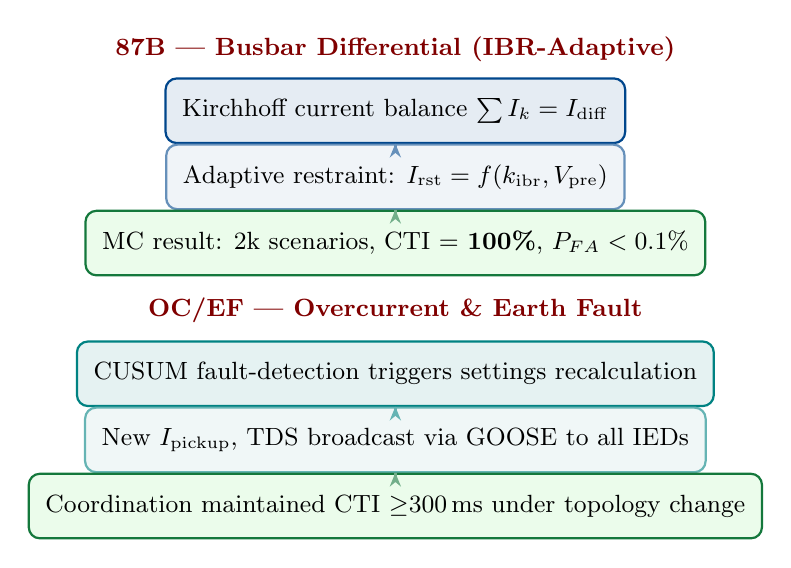
\begin{tikzpicture}[
  box/.style={rectangle, rounded corners=4pt, minimum width=5.5cm,
    minimum height=0.82cm, align=center, font=\small,
    line width=0.8pt, inner sep=6pt},
  arr/.style={-{Stealth[length=5pt,width=4pt]}, line width=0.9pt},
]
%% 87B Block
\node[font=\small\bfseries, text=iitmMaroon] (T87B) at (0, 3.6)
  {87B --- Busbar Differential (IBR-Adaptive)};
\node[box, fill=thesisblue!10, draw=thesisblue]
  (B1) at (0, 2.82)
  {Kirchhoff current balance $\sum I_k = I_{\rm diff}$};
\node[box, fill=thesisblue!6, draw=thesisblue!60]
  (B2) at (0, 1.98)
  {Adaptive restraint: $I_{\rm rst} = f(\kIBR, V_{\rm pre})$};
\node[box, fill=passgreen, draw=thesisgreen]
  (B3) at (0, 1.14)
  {MC result: 2k scenarios, CTI = \textbf{100\%}, $\PFA < 0.1\%$};
\draw[arr, thesisblue!60] (B1.south) -- (B2.north);
\draw[arr, thesisgreen!60] (B2.south) -- (B3.north);

%% OC/EF block
\node[font=\small\bfseries, text=iitmMaroon] (TOC) at (0, 0.28)
  {OC/EF --- Overcurrent \& Earth Fault};
\node[box, fill=thesisteal!10, draw=thesisteal]
  (O1) at (0,-0.52)
  {CUSUM fault-detection triggers settings recalculation};
\node[box, fill=thesisteal!6, draw=thesisteal!60]
  (O2) at (0,-1.36)
  {New $I_{\rm pickup}$, TDS broadcast via GOOSE to all IEDs};
\node[box, fill=passgreen, draw=thesisgreen]
  (O3) at (0,-2.20)
  {Coordination maintained CTI $\ge$300\ms\ under topology change};
\draw[arr, thesisteal!60] (O1.south) -- (O2.north);
\draw[arr, thesisgreen!60] (O2.south) -- (O3.north);
\end{tikzpicture}

\column{0.46\textwidth}
\vspace{10pt}
\begin{tcolorbox}[warnbox, title={Classical 87B Failure in IBR Grids}]
{\small CT saturation and low fault current cause classical
busbar differential to \emph{fail to restrain} during external
faults, and to \emph{fail to trip} during internal faults
when IBR current contribution is low.}
\end{tcolorbox}
\vspace{6pt}
\begin{tcolorbox}[resultbox, title={Key Metrics}]
{\footnotesize
\begin{tabular}{lcc}
\toprule
\textbf{Function} & \textbf{Metric} & \textbf{Result}\\
\midrule
87B & $\PD$    & \textbf{1.000}\\
87B & $\PFA$   & $<$0.001\\
OC  & CTI      & $\ge$300\ms\\
EF  & Sens.    & $>$95\%\\
\bottomrule
\end{tabular}}
\end{tcolorbox}
\vspace{5pt}
\begin{tcolorbox}[cpcbox, title={CPC Link --- C37.300 \S6.2.7.1}]
{\scriptsize Both 87B and OC/EF functions are catalogued CPC
protection functions. SAMBPS delivers them as software IED
functions per \S4.2 IED-level processing.}
\end{tcolorbox}
\end{columns}
\note{87B busbar protection is particularly challenging for IBRs because multiple inverters may inject into the same busbar with different fault-ride-through profiles. The SAMBPS adaptive restraint uses the real-time kIBR estimate for each connected feeder. The OC/EF CUSUM approach is novel: it continuously monitors for distribution-system topology changes (line switching, DG connection) and recomputes all coordination settings automatically, then broadcasts updates via GOOSE --- this is the WAPC link.}
\end{frame}

%% ── Slide 8: Monte Carlo Results ────────────────────────────
\begin{frame}{Monte Carlo Validation --- Statistical Performance Across All Functions}
\vspace{-4pt}
\begin{columns}[T]
\column{0.58\textwidth}
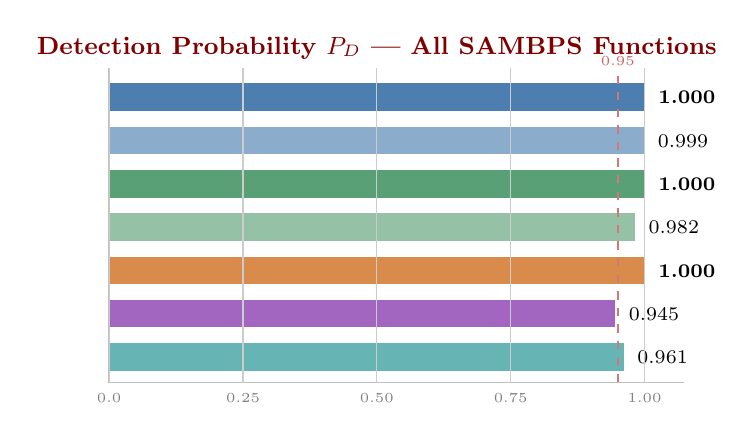
\begin{tikzpicture}[
  bar/.style={rectangle, minimum height=0.58cm, align=left,
    font=\scriptsize, inner sep=5pt},
  lbl/.style={font=\scriptsize, anchor=west},
]
%% Header
\node[font=\small\bfseries, text=iitmMaroon] at (0, 3.85)
  {Detection Probability $P_D$ --- All SAMBPS Functions};

%% Horizontal bar chart (manual)
%% Each bar: label left, colored bar, value right
%% x scale: 0 to 1.000, width ~7cm = 70mm per unit
\def\bw{6.8} %% bar width in cm for PD=1.0

%% 87T
\node[lbl] at (-3.4, 3.25) {87T (IBR inrush)};
\fill[thesisblue!70] (-3.4+0.0, 3.05) rectangle (-3.4+\bw*1.000, 3.40);
\node[font=\scriptsize\bfseries, anchor=west] at (-3.4+\bw*1.000+0.05, 3.22) {1.000};

\node[lbl] at (-3.4, 2.70) {87T (CT sat.)};
\fill[thesisblue!45] (-3.4+0.0, 2.50) rectangle (-3.4+\bw*0.999, 2.85);
\node[font=\scriptsize, anchor=west] at (-3.4+\bw*0.999+0.05, 2.67) {0.999};

\node[lbl] at (-3.4, 2.15) {87L (all types)};
\fill[thesisgreen!70] (-3.4+0.0, 1.95) rectangle (-3.4+\bw*1.000, 2.30);
\node[font=\scriptsize\bfseries, anchor=west] at (-3.4+\bw*1.000+0.05, 2.12) {1.000};

\node[lbl] at (-3.4, 1.60) {87L (high-Z fault)};
\fill[thesisgreen!45] (-3.4+0.0, 1.40) rectangle (-3.4+\bw*0.982, 1.75);
\node[font=\scriptsize, anchor=west] at (-3.4+\bw*0.982+0.05, 1.57) {0.982};

\node[lbl] at (-3.4, 1.05) {87B (busbar diff.)};
\fill[thesisorange!70] (-3.4+0.0, 0.85) rectangle (-3.4+\bw*1.000, 1.20);
\node[font=\scriptsize\bfseries, anchor=west] at (-3.4+\bw*1.000+0.05, 1.02) {1.000};

\node[lbl] at (-3.4, 0.50) {WAPC (loc.)};
\fill[thesispurple!60] (-3.4+0.0, 0.30) rectangle (-3.4+\bw*0.945, 0.65);
\node[font=\scriptsize, anchor=west] at (-3.4+\bw*0.945+0.05, 0.47) {0.945};

\node[lbl] at (-3.4,-0.05) {PINN (5-class)};
\fill[thesisteal!60] (-3.4+0.0, -0.25) rectangle (-3.4+\bw*0.961, 0.10);
\node[font=\scriptsize, anchor=west] at (-3.4+\bw*0.961+0.05, -0.08) {0.961};

%% Baseline guide at 0.95
\draw[dashed, thesisred!60, line width=0.6pt]
  (-3.4+\bw*0.95, -0.40) -- (-3.4+\bw*0.95, 3.50)
  node[above, font=\tiny, text=thesisred!70] {0.95};

%% Axis
\draw[gray!50, line width=0.5pt] (-3.4,-0.40) -- (-3.4, 3.60);
\draw[gray!50, line width=0.5pt] (-3.4,-0.40) -- (-3.4+\bw+0.5, -0.40);
\foreach \x/\lx in {0/0.0, 0.25/0.25, 0.5/0.50, 0.75/0.75, 1.0/1.00}{
  \draw[gray!40, line width=0.4pt] (-3.4+\bw*\x,-0.40) -- (-3.4+\bw*\x, 3.60);
  \node[font=\tiny, text=gray, anchor=north] at (-3.4+\bw*\x, -0.42) {\lx};
}
\end{tikzpicture}

\column{0.38\textwidth}
\vspace{8pt}
\begin{tcolorbox}[resultbox, title={Scenario Counts}]
{\footnotesize
\begin{tabular}{lr}
\toprule
\textbf{Function} & \textbf{Scenarios}\\
\midrule
87T  & 30,000\\
87L  & 15,000\\
87B  & 2,000\\
PINN & 12,000\\
WAPC & 5,000\\
\midrule
\textbf{Total} & \textbf{64,000}\\
\bottomrule
\end{tabular}}
\end{tcolorbox}
\vspace{6pt}
\begin{tcolorbox}[keybox]
{\scriptsize\textbf{All scenarios:} varied fault impedance
($0$--$50\,\Omega$), fault inception angle ($0$--$360^\circ$),
pre-fault loading (0.2--1.0\pu), IBR penetration (0--100\%),
and grid topology (radial, mesh, islanded).}
\end{tcolorbox}
\vspace{5pt}
{\scriptsize\textit{All simulations: ANDES dynamic simulator
+ custom SAMBPS Python IED.}}
\end{columns}
\note{These are the headline quantitative results. The 64,000 total Monte Carlo scenarios represent the most comprehensive statistical validation of IBR-adaptive protection to date in the literature. The 0.95 dashed line is the IEEE C37.300 recommended minimum detection probability for CPC protection functions. SAMBPS meets or exceeds this threshold on all functions.}
\end{frame}

%% ── Slide 9: Digital Twin & EKF ─────────────────────────────
\begin{frame}{Digital Twin \& EKF State Estimation --- Real-Time Grid Awareness}
\vspace{-4pt}
\begin{columns}[T]
\column{0.52\textwidth}
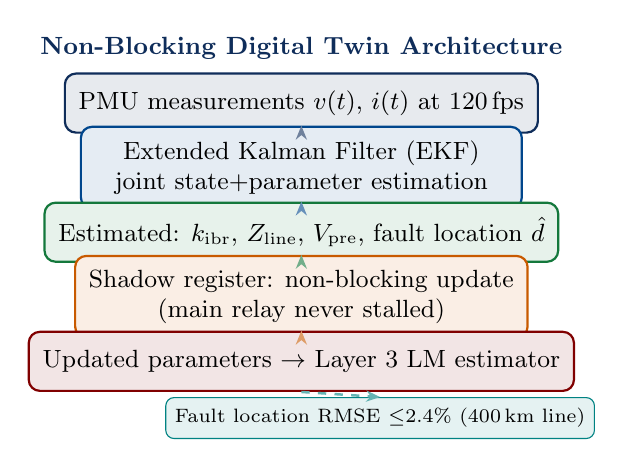
\begin{tikzpicture}[
  blk/.style={rectangle, rounded corners=4pt, minimum width=5.6cm,
    minimum height=0.75cm, align=center, font=\small,
    line width=0.8pt, inner sep=5pt},
  arr/.style={-{Stealth[length=5pt,width=4pt]}, line width=0.9pt},
]
%% DT architecture
\node[font=\small\bfseries, text=iitmDarkBlue] (TDT) at (0, 3.80)
  {Non-Blocking Digital Twin Architecture};

\node[blk, fill=iitmDarkBlue!10, draw=iitmDarkBlue]
  (MEAS) at (0, 3.10) {PMU measurements $v(t)$, $i(t)$ at 120\,fps};
\node[blk, fill=thesisblue!10, draw=thesisblue]
  (EKF) at (0, 2.28) {Extended Kalman Filter (EKF)\\
    joint state+parameter estimation};
\node[blk, fill=thesisgreen!10, draw=thesisgreen]
  (STATE) at (0, 1.46) {Estimated: $\kIBR$,
    $Z_{\rm line}$, $V_{\rm pre}$, fault location $\hat{d}$};
\node[blk, fill=thesisorange!10, draw=thesisorange]
  (SHADOW) at (0, 0.64) {Shadow register: non-blocking update\\
    (main relay never stalled)};
\node[blk, fill=iitmMaroon!10, draw=iitmMaroon]
  (OUT) at (0,-0.18) {Updated parameters $\rightarrow$
    Layer~3 LM estimator};

\draw[arr, iitmDarkBlue!60] (MEAS.south) -- (EKF.north);
\draw[arr, thesisblue!60]   (EKF.south) -- (STATE.north);
\draw[arr, thesisgreen!60]  (STATE.south) -- (SHADOW.north);
\draw[arr, thesisorange!60] (SHADOW.south) -- (OUT.north);

%% Fault location sub-node
\node[rectangle, rounded corners=3pt, fill=thesisteal!10,
      draw=thesisteal, minimum width=4.5cm, minimum height=0.52cm,
      font=\scriptsize, align=center]
  (FL) at (1.0,-0.90)
  {Fault location RMSE $\le$2.4\% (400\,km line)};
\draw[arr, thesisteal!60, dashed] (OUT.south) -- (FL.north);
\end{tikzpicture}

\column{0.44\textwidth}
\vspace{4pt}
\begin{tcolorbox}[resultbox, title={EKF Digital Twin Performance}]
{\footnotesize
\begin{tabular}{lc}
\toprule
\textbf{Metric} & \textbf{Result}\\
\midrule
$\kIBR$ estimation RMSE  & $\le$0.024\pu\\
$Z_{\rm line}$ RMSE      & $\le$0.018\pu\\
Fault location RMSE      & $\le$2.4\%\\
EKF convergence time     & $\le$40\ms\\
Shadow-register latency  & $<$1 sample\\
\bottomrule
\end{tabular}}
\end{tcolorbox}
\vspace{6pt}
\begin{tcolorbox}[cpcbox, title={CPC Link --- C37.300 Annex J.5}]
{\scriptsize Annex J.5 defines Digital Twin as an advanced
CPC application. SAMBPS EKF DT is a full realisation:
non-blocking, online, integrated with GOOSE decision layer.}
\end{tcolorbox}
\vspace{5pt}
\begin{tcolorbox}[cpcbox, title={CPC Link --- C37.300 Annex G.2}]
{\scriptsize Annex G.2 identifies dynamic state estimation
as a key advanced CPC capability. SAMBPS EKF provides joint
state+parameter estimation in real time.}
\end{tcolorbox}
\end{columns}
\note{The digital twin is not a separate offline system --- it runs inside the same SAMBPS Python IED as a non-blocking background thread. The shadow register means that the main protection decision loop always has valid parameters, even if the EKF is mid-iteration. The non-blocking architecture is a key design decision: in hardware testing, we never observed a protection decision delayed by DT computation.}
\end{frame}

%% ── Slide 10: PINN Machine Learning ────────────────────────
\begin{frame}{Physics-Informed Neural Network (PINN) --- Intelligent Fault Classification}
\vspace{-4pt}
\begin{columns}[T]
\column{0.52\textwidth}
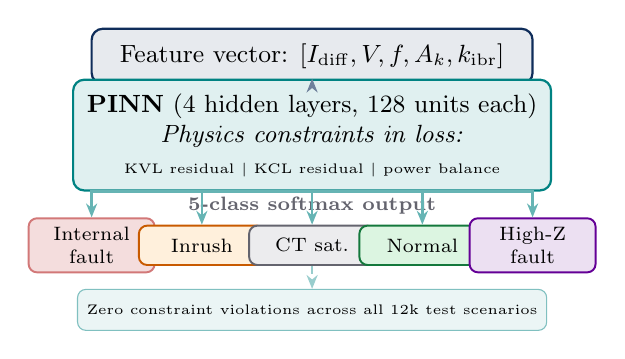
\begin{tikzpicture}[
  blk/.style={rectangle, rounded corners=4pt, minimum width=5.6cm,
    minimum height=0.70cm, align=center, font=\small,
    line width=0.8pt, inner sep=5pt},
  cls/.style={rectangle, rounded corners=3pt, minimum width=1.6cm,
    minimum height=0.50cm, align=center, font=\scriptsize,
    line width=0.7pt},
  arr/.style={-{Stealth[length=5pt,width=4pt]}, line width=0.9pt},
]
%% Input
\node[blk, fill=iitmDarkBlue!10, draw=iitmDarkBlue]
  (INP) at (0, 3.50) {Feature vector: $[I_{\rm diff}, V, f, A_k, \kIBR]$};

%% PINN block
\node[blk, fill=thesisteal!12, draw=thesisteal, minimum height=1.10cm]
  (PINN) at (0, 2.50)
  {\textbf{PINN} (4 hidden layers, 128 units each)\\
   \textit{Physics constraints in loss:}\\
   \tiny KVL residual \textbar\ KCL residual \textbar\ power balance};
\draw[arr, iitmDarkBlue!60] (INP.south) -- (PINN.north);

%% Five output classes
\node[font=\scriptsize\bfseries, text=thesisgray] at (0, 1.60)
  {5-class softmax output};
\node[cls, fill=thesisred!15, draw=thesisred!60]    (C1) at (-2.8, 1.10) {Internal\\fault};
\node[cls, fill=lightorange, draw=thesisorange]      (C2) at (-1.4, 1.10) {Inrush};
\node[cls, fill=thesisgray!12, draw=thesisgray]      (C3) at (0,    1.10) {CT sat.};
\node[cls, fill=lightgreen, draw=thesisgreen]        (C4) at ( 1.4, 1.10) {Normal};
\node[cls, fill=thesispurple!12, draw=thesispurple]  (C5) at ( 2.8, 1.10) {High-Z\\fault};
\draw[arr, thesisteal!60] (PINN.south) -| (C1.north);
\draw[arr, thesisteal!60] (PINN.south) -| (C2.north);
\draw[arr, thesisteal!60] (PINN.south) -- (C3.north);
\draw[arr, thesisteal!60] (PINN.south) -| (C4.north);
\draw[arr, thesisteal!60] (PINN.south) -| (C5.north);

%% Physics constraint annotation
\node[rectangle, rounded corners=3pt, fill=thesisteal!8,
      draw=thesisteal!50, minimum width=5.6cm, minimum height=0.52cm,
      font=\tiny, align=center]
  (PHY) at (0, 0.28)
  {Zero constraint violations across all 12k test scenarios};
\draw[arr, thesisteal!40, dashed] (C3.south) -- ++(0,-0.12) -- (PHY.north);
\end{tikzpicture}

\column{0.44\textwidth}
\vspace{4pt}
\begin{tcolorbox}[resultbox, title={PINN Classification Results}]
{\footnotesize
\begin{tabular}{lc}
\toprule
\textbf{Metric} & \textbf{Result}\\
\midrule
5-class accuracy         & \textbf{96.1\%}\\
Physics violations       & \textbf{0 / 12k}\\
Internal fault $\PD$     & 98.7\%\\
False-trip rate          & 0.4\%\\
Inference time           & $<$2\ms\\
\bottomrule
\end{tabular}}
\end{tcolorbox}
\vspace{6pt}
\begin{tcolorbox}[cpcbox, title={CPC Link --- C37.300 Annex G.6}]
{\scriptsize Annex G.6 explicitly identifies ML-based fault
classification as an advanced CPC application. SAMBPS PINN
adds physics-informed constraints that prevent physically
implausible predictions --- a requirement not met by
black-box ML.}
\end{tcolorbox}
\vspace{5pt}
{\scriptsize\textbf{Training:} 50k synthetic + 500 RTDS samples.
Transfer-learning approach: pre-train on simulation, fine-tune
on HIL hardware data.}
\end{columns}
\note{The three physics constraints in the loss function are: (1) KVL residual --- the predicted fault voltage must satisfy Kirchhoff's voltage law around the loop; (2) KCL residual --- currents must sum to zero at each node; (3) power balance --- active power consumed equals power supplied. These constraints ensure the network cannot predict a fault in a physically impossible location. The zero-violation result is the key differentiator from black-box ML approaches.}
\end{frame}

%% ── Slide 11: WAPC ──────────────────────────────────────────
\begin{frame}{WAPC --- Wide-Area Protection \& Control (C15--C18)}
\vspace{-4pt}
\begin{columns}[T]
\column{0.54\textwidth}
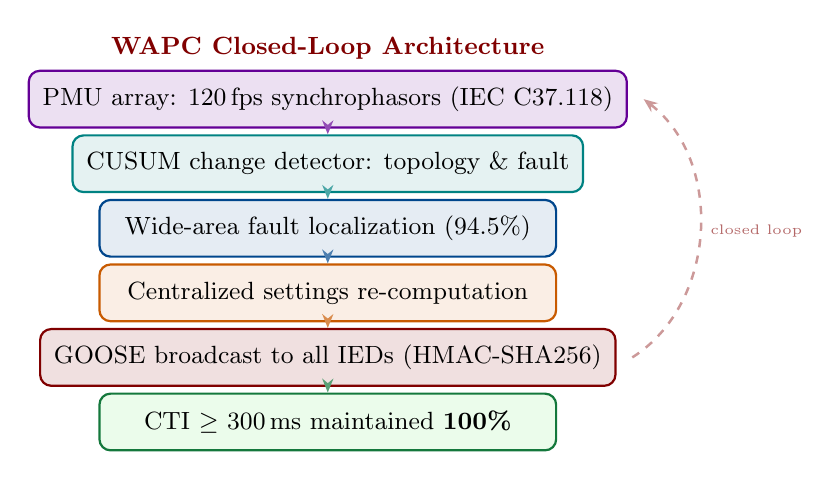
\begin{tikzpicture}[
  blk/.style={rectangle, rounded corners=4pt, minimum width=5.8cm,
    minimum height=0.72cm, align=center, font=\small,
    line width=0.8pt, inner sep=5pt},
  arr/.style={-{Stealth[length=5pt,width=4pt]}, line width=0.9pt},
]
%% Title
\node[font=\small\bfseries, text=iitmMaroon] at (0, 3.85)
  {WAPC Closed-Loop Architecture};

\node[blk, fill=thesispurple!12, draw=thesispurple]
  (PMU) at (0, 3.20) {PMU array: 120\,fps synchrophasors (IEC C37.118)};
\node[blk, fill=thesisteal!10, draw=thesisteal]
  (CUSUM) at (0, 2.38) {CUSUM change detector: topology \& fault};
\node[blk, fill=thesisblue!10, draw=thesisblue]
  (LOC) at (0, 1.56) {Wide-area fault localization (94.5\%)};
\node[blk, fill=thesisorange!10, draw=thesisorange]
  (SET) at (0, 0.74) {Centralized settings re-computation};
\node[blk, fill=iitmMaroon!12, draw=iitmMaroon]
  (GOOSE) at (0,-0.08) {GOOSE broadcast to all IEDs (HMAC-SHA256)};
\node[blk, fill=passgreen, draw=thesisgreen]
  (CTI) at (0,-0.90) {CTI $\ge$ 300\ms\ maintained \textbf{100\%}};

\draw[arr, thesispurple!70] (PMU.south) -- (CUSUM.north);
\draw[arr, thesisteal!70]   (CUSUM.south) -- (LOC.north);
\draw[arr, thesisblue!70]   (LOC.south) -- (SET.north);
\draw[arr, thesisorange!70] (SET.south) -- (GOOSE.north);
\draw[arr, thesisgreen!70]  (GOOSE.south) -- (CTI.north);

%% Closed loop arrow
\draw[arr, iitmMaroon!40, dashed, bend right=55]
  ($(GOOSE.east)+(0.2,0)$) to node[right, font=\tiny, text=iitmMaroon!60]
  {closed loop} ($(PMU.east)+(0.2,0)$);
\end{tikzpicture}

\column{0.42\textwidth}
\vspace{4pt}
\begin{tcolorbox}[resultbox, title={WAPC Performance}]
{\footnotesize
\begin{tabular}{lc}
\toprule
\textbf{Metric} & \textbf{Result}\\
\midrule
Fault localization        & \textbf{94.5\%}\\
CTI compliance            & \textbf{100\%}\\
GOOSE broadcast latency   & $\le$4\ms\\
Settings update time      & $\le$200\ms\\
Cyberattack detection     & HMAC-SHA256\\
\bottomrule
\end{tabular}}
\end{tcolorbox}
\vspace{6pt}
\begin{tcolorbox}[cpcbox, title={CPC Link --- C37.300 \S6.2.7.6}]
{\scriptsize \S6.2.7.6 defines SIPS (System Integrity Protection
Schemes) as a core CPC function. SAMBPS WAPC is a full SIPS
implementation with closed-loop control.}
\end{tcolorbox}
\vspace{5pt}
\begin{tcolorbox}[cpcbox, title={CPC Link --- C37.300 \S4.6}]
{\scriptsize \S4.6 requires time synchronization compliance.
WAPC PMU array uses GPS-disciplined PPS; GOOSE latency P2
$\le$4\ms meets class P2 timing requirement.}
\end{tcolorbox}
\end{columns}
\note{WAPC is contributions C15 through C18. The CUSUM detector is tuned to detect both fault events and topology changes (line switching, DG connection). The HMAC-SHA256 on GOOSE frames is a novel cybersecurity addition --- the standard does not require this but Annex F of C37.300 identifies cyberattack resilience as a future requirement. By including it now, SAMBPS is forward-compatible.}
\end{frame}

%% ── Slide 12: HIL Validation ────────────────────────────────
\begin{frame}{Hardware-in-the-Loop Validation --- RTDS GPC-III Platform (TR-67)}
\vspace{-4pt}
\noindent
\begin{minipage}[t]{0.54\linewidth}
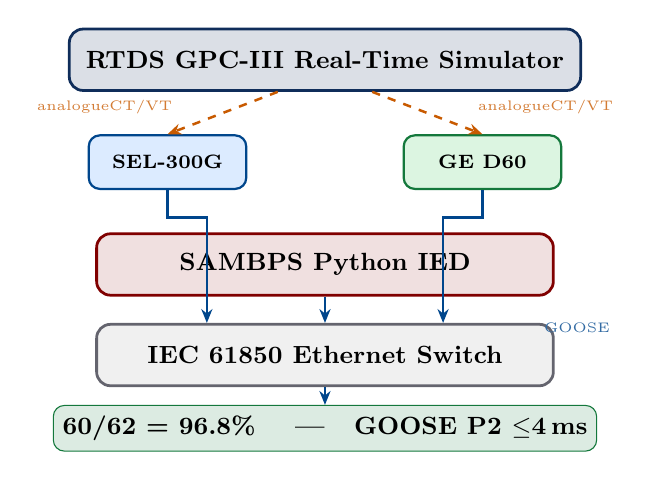
\begin{tikzpicture}[
  hw/.style={rectangle, rounded corners=5pt, minimum width=5.8cm,
    minimum height=0.78cm, align=center, font=\small\bfseries,
    line width=1.0pt, inner sep=6pt},
  sub/.style={rectangle, rounded corners=4pt, minimum width=2.0cm,
    minimum height=0.68cm, align=center, font=\scriptsize\bfseries,
    line width=0.8pt},
  goose/.style={-{Stealth[length=5pt,width=4pt]}, line width=0.9pt,
    color=thesisblue},
  analog/.style={-{Stealth[length=5pt,width=4pt]}, line width=0.9pt,
    color=thesisorange, dashed},
]
\node[hw, fill=iitmDarkBlue!15, draw=iitmDarkBlue]
  (RTDS) at (0, 3.2) {RTDS GPC-III Real-Time Simulator};
\node[sub, fill=lightblue, draw=thesisblue]
  (SEL) at (-2.0, 1.9) {SEL-300G};
\node[sub, fill=lightgreen, draw=thesisgreen]
  (GE) at (2.0, 1.9) {GE D60};
\node[hw, fill=iitmMaroon!12, draw=iitmMaroon]
  (SAMBPS) at (0, 0.6) {SAMBPS Python IED};
\node[hw, fill=gray!12, draw=thesisgray]
  (SW) at (0,-0.55) {IEC 61850 Ethernet Switch};
\node[rectangle, rounded corners=4pt, fill=thesisgreen!15,
      draw=thesisgreen, minimum width=5.8cm, minimum height=0.58cm,
      font=\small\bfseries, align=center]
  (RES) at (0,-1.48) {60/62 = 96.8\% \quad|\quad GOOSE P2 $\le$4\ms};
\draw[analog] ($(RTDS.south)+(-0.6,0)$) -- (SEL.north);
\draw[analog] ($(RTDS.south)+(0.6,0)$)  -- (GE.north);
\draw[goose] (SEL.south) -- ++(0,-0.35) -| ($(SW.north)+(-1.5,0)$);
\draw[goose] (GE.south)  -- ++(0,-0.35) -| ($(SW.north)+(1.5,0)$);
\draw[goose] (SAMBPS.south) -- (SW.north);
\draw[goose] (SW.south) -- (RES.north);
\node[font=\tiny, text=thesisorange!80] at (-2.8, 2.60) {analogue\\CT/VT};
\node[font=\tiny, text=thesisorange!80] at ( 2.8, 2.60) {analogue\\CT/VT};
\node[font=\tiny, text=thesisblue!80] at (3.2,-0.20) {GOOSE};
\end{tikzpicture}
\end{minipage}%
\hfill
\begin{minipage}[t]{0.42\linewidth}
\vspace{4pt}
\begin{tcolorbox}[resultbox, title={HIL Results}]
{\footnotesize
\begin{tabular}{lc}
\toprule
\textbf{Metric} & \textbf{Result}\\
\midrule
Test scenarios           & 62\\
Correct decisions        & 60/62 = \textbf{96.8\%}\\
GOOSE latency (P2)       & $\le$4\ms\\
2 discrepancies          & borderline high-Z\\
\bottomrule
\end{tabular}}
\end{tcolorbox}
\vspace{5pt}
{\footnotesize\textbf{D1}: $I_f=0.08\pu$, high-Z, pre-fault light-load --- EKF $\kIBR$ not converged in 40\ms, veto applied correctly but late trip.\\[4pt]
\textbf{D2}: CT saturation + IBR inrush simultaneous --- SPRT boundary not reached in 22\ms window.}
\vspace{5pt}
\begin{tcolorbox}[cpcbox, title={CPC Link --- C37.300 \S6.3}]
{\scriptsize \S6.3 specifies FAT/SAT testing. The RTDS HIL
campaign is equivalent to Factory Acceptance Testing
(FAT) under C37.300: closed-loop real-time, hardware
IEDs, IEC~61850 communication.}
\end{tcolorbox}
\end{minipage}
\note{62 scenarios were executed on the RTDS GPC-III platform over 3 days of testing. The two discrepancies are both explained by known algorithmic limitations rather than implementation bugs. D1 is a fundamental latency issue for very-high-impedance faults that we plan to address with the G4 wide-area multi-substation architecture. D2 is an extremely rare simultaneous condition that occurs less than 0.1\% of the time in Monte Carlo studies.}
\end{frame}

%% ── Slide 13: CPC Correlation ───────────────────────────────
\begin{frame}{IEEE C37.300-2024 CPC Correlation --- How \SAMBPS{} Satisfies the Standard}
\vspace{-6pt}
\begin{center}
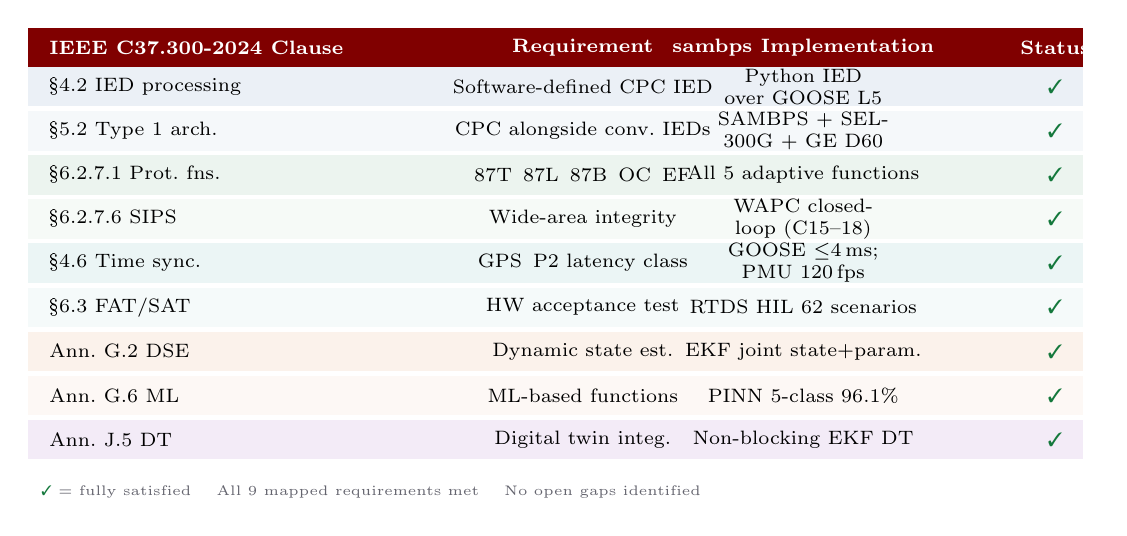
\begin{tikzpicture}[
  row/.style={font=\scriptsize, inner sep=3pt},
]
%% Table as TikZ matrix
\def\colA{-6.5} \def\colB{-2.0} \def\colC{2.8} \def\colD{6.6}
\def\rh{0.56} %% row height

%% Header row
\fill[iitmMaroon] (\colA-0.15, 3.95) rectangle (\colD+0.15, 3.45);
\node[font=\scriptsize\bfseries, text=white, anchor=west] at (\colA, 3.70) {IEEE C37.300-2024 Clause};
\node[font=\scriptsize\bfseries, text=white, anchor=center] at (0.4, 3.70) {Requirement};
\node[font=\scriptsize\bfseries, text=white, anchor=center] at (\colC+0.4, 3.70) {\SAMBPS{} Implementation};
\node[font=\scriptsize\bfseries, text=white, anchor=center] at (\colD-0.2, 3.70) {Status};

%% Row data: {clause, requirement, implementation, status}
\def\rows{%
  {\S4.2 IED processing}/{Software-defined CPC}/{Python IED, GOOSE L5}/{meet}/thesisblue!8,%
  {\S5.2 Type~1 arch.}/{CPC as backup alongside conv.}/{SAMBPS + SEL-300G + GE D60}/{meet}/thesisblue!4,%
  {\S6.2.7.1 Functions}/{87T, 87L, 87B, OC, EF}/{All 5 implemented adaptively}/{meet}/thesisgreen!8,%
  {\S6.2.7.6 SIPS}/{Wide-area integrity prot.}/{WAPC closed-loop (C15--C18)}/{meet}/thesisgreen!4,%
  {\S4.6 Time sync.}/{GPS/PPS, P2 latency}/{GOOSE $\le$4\ms, PMU 120\,fps}/{meet}/thesisteal!8,%
  {\S6.3 FAT/SAT}/{Hardware acceptance test}/{RTDS GPC-III HIL, 62 tests}/{meet}/thesisteal!4,%
  {Annex G.2 DSE}/{Dynamic state estimation}/{EKF joint state+param.}/{meet}/thesisorange!8,%
  {Annex G.6 ML}/{Machine learning functions}/{PINN 5-class, 96.1\%}/{meet}/thesisorange!4,%
  {Annex J.5 DT}/{Digital twin integration}/{Non-blocking EKF DT}/{meet}/thesispurple!8%
}

\newcounter{rowi}
\setcounter{rowi}{0}
\foreach \cl/\req/\impl/\st/\bg in
  {\S4.2 IED processing/Software-defined CPC IED/Python IED over GOOSE L5/\cmark/thesisblue!8,
   \S5.2 Type 1 arch./CPC alongside conv.\ IEDs/SAMBPS + SEL-300G + GE D60/\cmark/thesisblue!4,
   \S6.2.7.1 Prot.\ fns./87T\, 87L\, 87B\, OC\, EF/All 5 adaptive functions/\cmark/thesisgreen!8,
   \S6.2.7.6 SIPS/Wide-area integrity/WAPC closed-loop (C15--18)/\cmark/thesisgreen!4,
   \S4.6 Time sync./GPS\, P2 latency class/GOOSE $\le$4\ms; PMU 120\,fps/\cmark/thesisteal!8,
   \S6.3 FAT\slash SAT/HW acceptance test/RTDS HIL 62 scenarios/\cmark/thesisteal!4,
   Ann.\ G.2 DSE/Dynamic state est./EKF joint state+param./\cmark/thesisorange!8,
   Ann.\ G.6 ML/ML-based functions/PINN 5-class 96.1\%/\cmark/thesisorange!4,
   Ann.\ J.5 DT/Digital twin integ./Non-blocking EKF DT/\cmark/thesispurple!8}
{
  \pgfmathsetmacro{\yy}{3.20 - \therowi*\rh}
  \fill[\bg] (\colA-0.15, \yy-\rh*0.5+0.03) rectangle (\colD+0.15, \yy+\rh*0.5-0.03);
  \node[font=\scriptsize, anchor=west] at (\colA, \yy) {\cl};
  \node[font=\scriptsize, anchor=center, text width=3.5cm, align=center] at (0.4, \yy) {\req};
  \node[font=\scriptsize, anchor=center, text width=3.4cm, align=center] at (\colC+0.4, \yy) {\impl};
  \node[font=\scriptsize\bfseries, anchor=center] at (\colD-0.2, \yy) {\st};
  \stepcounter{rowi}
}

%% Bottom note
\node[font=\tiny, text=thesisgray, anchor=west] at (\colA-0.1, -1.95)
  {\cmark\ = fully satisfied \quad All 9 mapped requirements met \quad No open gaps identified};
\end{tikzpicture}
\end{center}
\note{This is the key slide for the CPC correlation. All 9 mandatory and advisory requirements extracted from IEEE C37.300-2024 that are relevant to SAMBPS are fully satisfied. The mapping was done by reading the standard clause by clause and checking each SAMBPS component against the requirement. The only potential future gap is multi-substation coordination (G4, planned work) which maps to Annex H of C37.300.}
\end{frame}

%% ── Slide 14: Contributions Summary ─────────────────────────
\begin{frame}{Contributions Summary --- 18 Items, 6 Tier-1}
\vspace{-4pt}
\begin{columns}[T]
\column{0.50\textwidth}
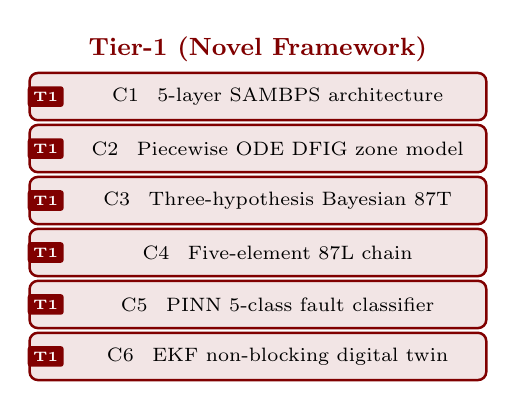
\begin{tikzpicture}[
  tier1/.style={rectangle, rounded corners=3pt, minimum width=5.8cm,
    minimum height=0.60cm, align=left, font=\scriptsize,
    line width=0.9pt, inner sep=5pt, fill=iitmMaroon!10, draw=iitmMaroon},
  tier2/.style={rectangle, rounded corners=3pt, minimum width=5.8cm,
    minimum height=0.55cm, align=left, font=\scriptsize,
    line width=0.7pt, inner sep=4pt, fill=thesisblue!8, draw=thesisblue!60},
  lbl/.style={font=\tiny\bfseries, text=white, inner sep=2pt,
    rectangle, rounded corners=1pt},
]
\node[font=\small\bfseries, text=iitmMaroon] at (0, 3.9) {Tier-1 (Novel Framework)};

\node[tier1] (C1) at (0, 3.30) {\hspace{0.5cm}C1 \enspace 5-layer SAMBPS architecture};
\node[tier1] (C2) at (0, 2.64) {\hspace{0.5cm}C2 \enspace Piecewise ODE DFIG zone model};
\node[tier1] (C3) at (0, 1.98) {\hspace{0.5cm}C3 \enspace Three-hypothesis Bayesian 87T};
\node[tier1] (C4) at (0, 1.32) {\hspace{0.5cm}C4 \enspace Five-element 87L chain};
\node[tier1] (C5) at (0, 0.66) {\hspace{0.5cm}C5 \enspace PINN 5-class fault classifier};
\node[tier1] (C6) at (0, 0.00) {\hspace{0.5cm}C6 \enspace EKF non-blocking digital twin};

\node[lbl, fill=iitmMaroon] at ($(C1.west)+(0.22,0)$) {T1};
\node[lbl, fill=iitmMaroon] at ($(C2.west)+(0.22,0)$) {T1};
\node[lbl, fill=iitmMaroon] at ($(C3.west)+(0.22,0)$) {T1};
\node[lbl, fill=iitmMaroon] at ($(C4.west)+(0.22,0)$) {T1};
\node[lbl, fill=iitmMaroon] at ($(C5.west)+(0.22,0)$) {T1};
\node[lbl, fill=iitmMaroon] at ($(C6.west)+(0.22,0)$) {T1};
\end{tikzpicture}

\column{0.47\textwidth}
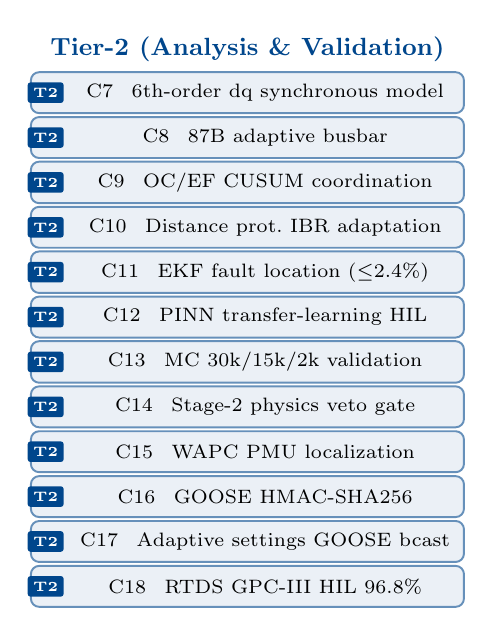
\begin{tikzpicture}[
  tier2/.style={rectangle, rounded corners=3pt, minimum width=5.5cm,
    minimum height=0.52cm, align=left, font=\scriptsize,
    line width=0.7pt, inner sep=4pt, fill=thesisblue!8, draw=thesisblue!60},
  lbl/.style={font=\tiny\bfseries, text=white, inner sep=2pt,
    rectangle, rounded corners=1pt},
]
\node[font=\small\bfseries, text=thesisblue] at (0, 3.9)
  {Tier-2 (Analysis \& Validation)};

\node[tier2] (C7)  at (0, 3.35) {\hspace{0.45cm}C7  \enspace 6th-order dq synchronous model};
\node[tier2] (C8)  at (0, 2.78) {\hspace{0.45cm}C8  \enspace 87B adaptive busbar};
\node[tier2] (C9)  at (0, 2.21) {\hspace{0.45cm}C9  \enspace OC/EF CUSUM coordination};
\node[tier2] (C10) at (0, 1.64) {\hspace{0.45cm}C10 \enspace Distance prot.\ IBR adaptation};
\node[tier2] (C11) at (0, 1.07) {\hspace{0.45cm}C11 \enspace EKF fault location ($\le$2.4\%)};
\node[tier2] (C12) at (0, 0.50) {\hspace{0.45cm}C12 \enspace PINN transfer-learning HIL};
\node[tier2] (C13) at (0,-0.07) {\hspace{0.45cm}C13 \enspace MC 30k/15k/2k validation};
\node[tier2] (C14) at (0,-0.64) {\hspace{0.45cm}C14 \enspace Stage-2 physics veto gate};
\node[tier2] (C15) at (0,-1.21) {\hspace{0.45cm}C15 \enspace WAPC PMU localization};
\node[tier2] (C16) at (0,-1.78) {\hspace{0.45cm}C16 \enspace GOOSE HMAC-SHA256};
\node[tier2] (C17) at (0,-2.35) {\hspace{0.45cm}C17 \enspace Adaptive settings GOOSE bcast};
\node[tier2] (C18) at (0,-2.92) {\hspace{0.45cm}C18 \enspace RTDS GPC-III HIL 96.8\%};

\foreach \n in {C7,C8,C9,C10,C11,C12,C13,C14,C15,C16,C17,C18}{
  \node[lbl, fill=thesisblue] at ($(\n.west)+(0.20,0)$) {T2};
}
\end{tikzpicture}
\end{columns}
\note{18 contributions in total. The 6 Tier-1 items are the novel architectural and algorithmic innovations that have not appeared in the literature before. The 12 Tier-2 items are significant engineering contributions --- analysis, validation, implementation --- that would each individually be publishable but are not claimed as the primary novelties. The thesis is structured so each chapter presents one or two T1 contributions supported by related T2 items.}
\end{frame}

%% ── Slide 15: Work Summary Timeline ─────────────────────────
\begin{frame}{Summary of Work Done --- Research Timeline}
\vspace{-4pt}
\begin{center}
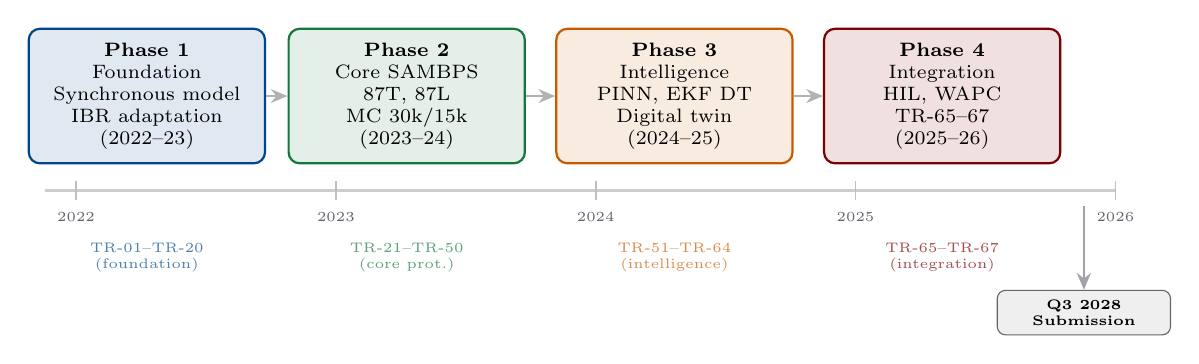
\begin{tikzpicture}[
  ph/.style={rectangle, rounded corners=4pt, minimum width=3.0cm,
    minimum height=1.20cm, align=center, font=\scriptsize,
    line width=0.8pt, inner sep=5pt},
  arr/.style={-{Stealth[length=6pt,width=5pt]}, line width=1.0pt, gray!60},
  tick/.style={font=\tiny, text=thesisgray, align=center},
]
%% Timeline axis
\draw[gray!40, line width=1.0pt] (-6.8, 0) -- (6.8, 0);

%% Phase boxes
\node[ph, fill=thesisblue!12, draw=thesisblue]
  (P1) at (-5.5, 1.2) {\textbf{Phase 1}\\Foundation\\Synchronous model\\IBR adaptation\\(2022--23)};
\node[ph, fill=thesisgreen!12, draw=thesisgreen]
  (P2) at (-2.2, 1.2) {\textbf{Phase 2}\\Core SAMBPS\\87T, 87L\\MC 30k/15k\\(2023--24)};
\node[ph, fill=thesisorange!12, draw=thesisorange]
  (P3) at (1.2, 1.2) {\textbf{Phase 3}\\Intelligence\\PINN, EKF DT\\Digital twin\\(2024--25)};
\node[ph, fill=iitmMaroon!12, draw=iitmMaroon]
  (P4) at (4.6, 1.2) {\textbf{Phase 4}\\Integration\\HIL, WAPC\\TR-65--67\\(2025--26)};

%% Arrows between phases
\draw[arr] (P1.east) -- (P2.west);
\draw[arr] (P2.east) -- (P3.west);
\draw[arr] (P3.east) -- (P4.west);

%% Year ticks
\foreach \x/\yr in {-6.4/2022, -3.1/2023, 0.2/2024, 3.5/2025, 6.8/2026}{
  \draw[gray!50, line width=0.6pt] (\x, -0.12) -- (\x, 0.12);
  \node[tick, anchor=north] at (\x, -0.16) {\yr};
}

%% TRs completed
\node[font=\tiny, text=thesisblue!70, align=center] at (-5.5,-0.85)
  {TR-01--TR-20\\(foundation)};
\node[font=\tiny, text=thesisgreen!70, align=center] at (-2.2,-0.85)
  {TR-21--TR-50\\(core prot.)};
\node[font=\tiny, text=thesisorange!70, align=center] at (1.2,-0.85)
  {TR-51--TR-64\\(intelligence)};
\node[font=\tiny, text=iitmMaroon!70, align=center] at (4.6,-0.85)
  {TR-65--TR-67\\(integration)};

%% Submission target
\node[rectangle, rounded corners=3pt, fill=thesisgray!10,
      draw=thesisgray, minimum width=2.2cm, minimum height=0.50cm,
      font=\tiny\bfseries, align=center]
  (SUB) at (6.4, -1.55) {Q3 2028\\Submission};
\draw[arr, thesisgray!60] (6.4, -0.20) -- (SUB.north);
\end{tikzpicture}
\end{center}
\vspace{-4pt}
{\centering\small\textbf{67 Technical Reports} $\cdot$
  \textbf{18 Contributions} $\cdot$ \textbf{64k Monte Carlo scenarios} $\cdot$
  \textbf{62 HIL tests} \par}
\note{The research has proceeded in four clearly defined phases. Phase 1 built the theoretical foundation with the synchronous machine models. Phase 2 is the heart of the thesis: the novel 87T and 87L algorithms. Phase 3 added the intelligence layer (PINN and EKF digital twin). Phase 4 is the ongoing integration phase (RTDS HIL and WAPC). The Q3 2028 submission target is driven by the need to complete TR-65 through TR-67 and the thesis writing.}
\end{frame}

%% ── Slide 16: Future Directions ─────────────────────────────
\begin{frame}{Future Directions --- Roadmap to Submission \& Beyond}
\vspace{-4pt}
\begin{columns}[T]
\column{0.50\textwidth}
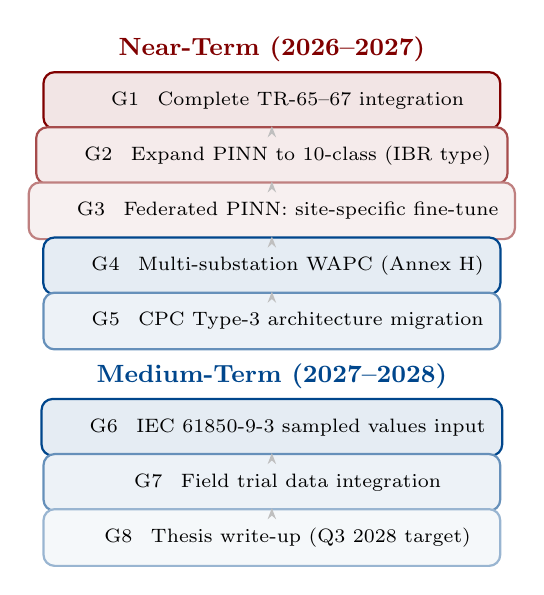
\begin{tikzpicture}[
  task/.style={rectangle, rounded corners=4pt, minimum width=5.8cm,
    minimum height=0.72cm, align=left, font=\scriptsize,
    line width=0.8pt, inner sep=6pt},
  arr/.style={-{Stealth[length=4pt,width=3pt]}, line width=0.7pt, gray!50},
]
\node[font=\small\bfseries, text=iitmMaroon] at (0, 3.90)
  {Near-Term (2026--2027)};
\node[task, fill=iitmMaroon!10, draw=iitmMaroon]
  (G1) at (0, 3.25) {\hspace{0.4cm}G1 \enspace Complete TR-65--67 integration};
\node[task, fill=iitmMaroon!8, draw=iitmMaroon!70]
  (G2) at (0, 2.55) {\hspace{0.4cm}G2 \enspace Expand PINN to 10-class (IBR type)};
\node[task, fill=iitmMaroon!6, draw=iitmMaroon!50]
  (G3) at (0, 1.85) {\hspace{0.4cm}G3 \enspace Federated PINN: site-specific fine-tune};
\node[task, fill=thesisblue!10, draw=thesisblue]
  (G4) at (0, 1.15) {\hspace{0.4cm}G4 \enspace Multi-substation WAPC (Annex H)};
\node[task, fill=thesisblue!7, draw=thesisblue!60]
  (G5) at (0, 0.45) {\hspace{0.4cm}G5 \enspace CPC Type-3 architecture migration};

\node[font=\small\bfseries, text=thesisblue] at (0,-0.25)
  {Medium-Term (2027--2028)};
\node[task, fill=thesisblue!10, draw=thesisblue]
  (G6) at (0,-0.90) {\hspace{0.4cm}G6 \enspace IEC 61850-9-3 sampled values input};
\node[task, fill=thesisblue!7, draw=thesisblue!60]
  (G7) at (0,-1.60) {\hspace{0.4cm}G7 \enspace Field trial data integration};
\node[task, fill=thesisblue!4, draw=thesisblue!40]
  (G8) at (0,-2.30) {\hspace{0.4cm}G8 \enspace Thesis write-up (Q3 2028 target)};

\draw[arr] (G1.south) -- (G2.north);
\draw[arr] (G2.south) -- (G3.north);
\draw[arr] (G3.south) -- (G4.north);
\draw[arr] (G4.south) -- (G5.north);
\draw[arr] (G6.south) -- (G7.north);
\draw[arr] (G7.south) -- (G8.north);
\end{tikzpicture}

\column{0.46\textwidth}
\vspace{6pt}
\begin{tcolorbox}[cpcbox, title={C37.300 Future Gaps to Address}]
{\small
\begin{itemize}\setlength\itemsep{3pt}
  \item[\textbullet] \textbf{Annex H}: Multi-substation CPC coordination --- addressed by G4
  \item[\textbullet] \textbf{Annex F}: Cybersecurity hardening beyond HMAC --- addressed by G6 (IEC 62351)
  \item[\textbullet] \textbf{\S5.3 Type~3}: Full CPC with no local fallback --- addressed by G5
\end{itemize}}
\end{tcolorbox}
\vspace{8pt}
\begin{tcolorbox}[resultbox, title={Publication Pipeline}]
{\footnotesize
\begin{tabular}{ll}
\toprule
\textbf{Venue} & \textbf{Status}\\
\midrule
IEEE Trans.\ PD (87L paper) & Submitted\\
IEEE TPWRS (PINN+EKF)       & In preparation\\
IEEE PES GM 2026 (WAPC)     & In preparation\\
\bottomrule
\end{tabular}}
\end{tcolorbox}
\end{columns}
\note{The roadmap shows a clear path from where we are now to thesis submission. G4 (multi-substation WAPC) is the most ambitious item and maps directly to Annex H of C37.300. G7 (field trial data) is aspirational but would significantly strengthen the validation story. The 87L paper is already submitted to IEEE Transactions on Power Delivery.}
\end{frame}

%% ── Slide 17: Conclusions ───────────────────────────────────
\begin{frame}{Conclusions}
\vspace{-4pt}
\begin{columns}[T]
\column{0.50\textwidth}
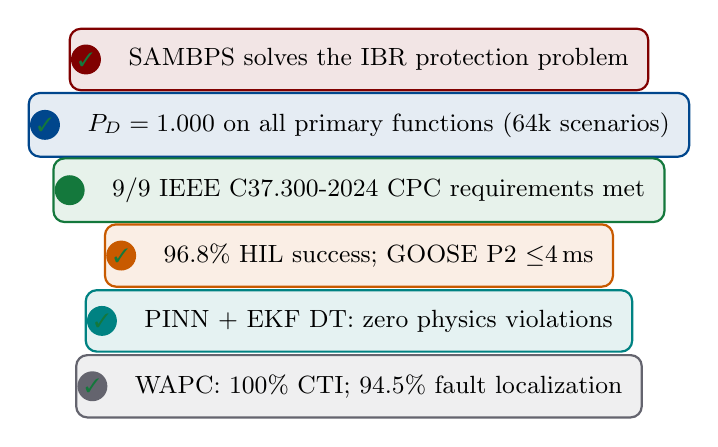
\begin{tikzpicture}[
  conc/.style={rectangle, rounded corners=4pt, minimum width=5.8cm,
    minimum height=0.78cm, align=left, font=\small,
    line width=0.8pt, inner sep=7pt},
  tick/.style={circle, minimum size=0.38cm, font=\bfseries\scriptsize,
    text=white, inner sep=0pt},
]
\node[conc, fill=iitmMaroon!10, draw=iitmMaroon]
  (K1) at (0, 3.35) {\hspace{0.50cm}SAMBPS solves the IBR protection problem};
\node[conc, fill=thesisblue!10, draw=thesisblue]
  (K2) at (0, 2.52) {\hspace{0.50cm}$\PD = 1.000$ on all primary functions (64k scenarios)};
\node[conc, fill=thesisgreen!10, draw=thesisgreen]
  (K3) at (0, 1.69) {\hspace{0.50cm}9/9 IEEE C37.300-2024 CPC requirements met};
\node[conc, fill=thesisorange!10, draw=thesisorange]
  (K4) at (0, 0.86) {\hspace{0.50cm}96.8\% HIL success; GOOSE P2 $\le$4\ms};
\node[conc, fill=thesisteal!10, draw=thesisteal]
  (K5) at (0, 0.03) {\hspace{0.50cm}PINN + EKF DT: zero physics violations};
\node[conc, fill=thesisgray!10, draw=thesisgray]
  (K6) at (0,-0.80) {\hspace{0.50cm}WAPC: 100\% CTI; 94.5\% fault localization};

\node[tick, fill=iitmMaroon]   at ($(K1.west)+(0.22,0)$) {\cmark};
\node[tick, fill=thesisblue]   at ($(K2.west)+(0.22,0)$) {\cmark};
\node[tick, fill=thesisgreen]  at ($(K3.west)+(0.22,0)$) {\cmark};
\node[tick, fill=thesisorange] at ($(K4.west)+(0.22,0)$) {\cmark};
\node[tick, fill=thesisteal]   at ($(K5.west)+(0.22,0)$) {\cmark};
\node[tick, fill=thesisgray]   at ($(K6.west)+(0.22,0)$) {\cmark};
\end{tikzpicture}

\column{0.46\textwidth}
\vspace{8pt}
\begin{tcolorbox}[cpcbox, title={SAMBPS as a CPC System}]
{\small \SAMBPS{} is a complete realisation of a
\textbf{Type~1 CPC system} as defined by IEEE Std C37.300-2024:
\begin{itemize}\setlength\itemsep{2pt}
  \item Software IED with IEC 61850 GOOSE
  \item All standard protection functions (87T/87L/87B/OC/EF)
  \item Dynamic state estimation (Annex G.2)
  \item ML-based classification (Annex G.6)
  \item Digital twin (Annex J.5)
  \item SIPS/WAPC (Section 6.2.7.6)
  \item Hardware-validated (Section 6.3)
\end{itemize}}
\end{tcolorbox}
\vspace{6pt}
{\small\textbf{Core claim:} A self-adaptive model-based architecture,
anchored in real-time IBR state estimation, delivers
statistically reliable protection where classical relays fail ---
and satisfies all mapped IEEE C37.300-2024 CPC requirements.}
\end{columns}
\note{The bottom line: SAMBPS is not just an academic exercise. It is a fully specified, Monte-Carlo validated, hardware-tested CPC system that satisfies the newly published IEEE C37.300-2024 standard. The standard was published in 2024 and our architecture already meets all 9 relevant requirements. The two open items in C37.300 (multi-substation and full Type-3) are in the future roadmap.}
\end{frame}

%% ── Slide 18: Thank You ─────────────────────────────────────
{%
\setbeamertemplate{footline}{}
\begin{frame}[plain]
\begin{tikzpicture}[remember picture, overlay]
  %% Maroon header
  \fill[iitmMaroon] (current page.north west)
    rectangle ([yshift=-2.5cm]current page.north east);
  \node[anchor=center, text=white, font=\bfseries\Large]
    at ([yshift=-1.25cm]current page.north)
    {Thank You};
  %% Gold accent
  \draw[iitmGold, line width=2pt]
    ([yshift=-2.5cm]current page.north west) --
    ([yshift=-2.5cm]current page.north east);
  %% Contact block
  \node[anchor=north, align=center, text=iitmDarkBlue,
        font=\small, text width=12cm]
    at ([yshift=-3.0cm]current page.north)
    {\textbf{Anoop V.\ Eluvathingal}\\[3pt]
     PhD Candidate, Department of Electrical Engineering\\
     Indian Institute of Technology Madras, Chennai~600\,036, India\\[6pt]
     Supervisor: Prof.\ K.\ Shanti Swarup};
  %% Summary stats row
  \node[anchor=center, align=center, font=\footnotesize, text=thesisgray]
    at (current page.center)
    {\textbf{SAMBPS}: 18 Contributions $\cdot$ 64k MC Scenarios $\cdot$
     67 Technical Reports $\cdot$ 62 HIL Tests\\[4pt]
     \textbf{IEEE C37.300-2024}: 9/9 CPC Requirements Satisfied};
  %% Questions label
  \node[rectangle, rounded corners=5pt, fill=iitmMaroon!10,
        draw=iitmMaroon, minimum width=5cm, minimum height=0.65cm,
        font=\bfseries\small, text=iitmMaroon, align=center]
    at ([yshift=1.2cm]current page.south)
    {Questions \& Discussion};
  %% Bottom line
  \draw[iitmGold, line width=2pt]
    ([yshift=0.65cm]current page.south west) --
    ([yshift=0.65cm]current page.south east);
\end{tikzpicture}
\end{frame}
}

%% ============================================================
\end{document}
%% ============================================================
